\begin{figure*}[t]
  \centering
  \begin{minipage}[t]{0.32\textwidth}
    \centering
    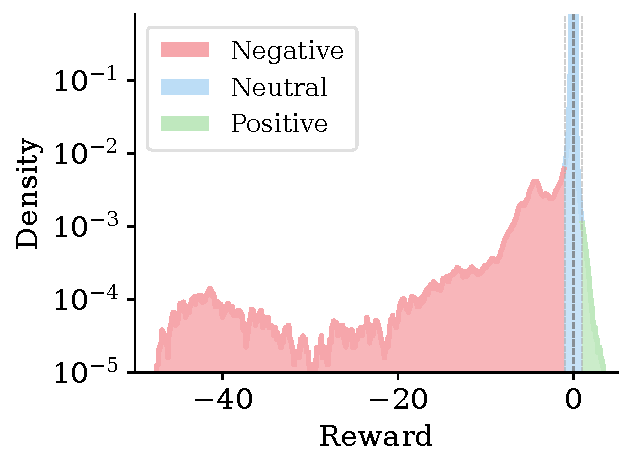
\includegraphics[width=\linewidth]{figures/fig3a_reward_distribution.pdf}\\[-0.5ex]
    \textbf{(a)}
  \end{minipage}\hfill
  \begin{minipage}[t]{0.32\textwidth}
    \centering
    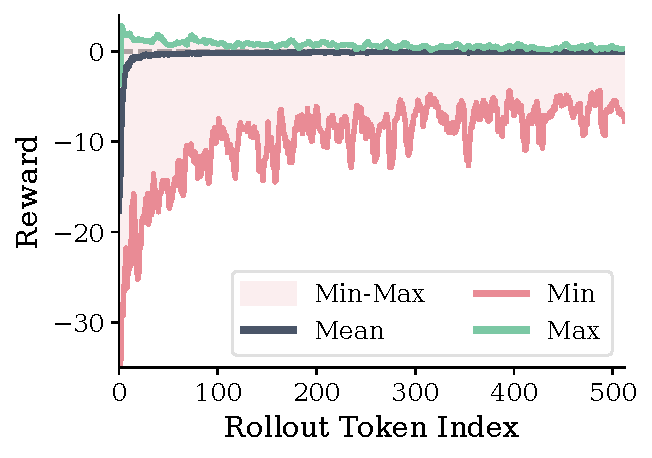
\includegraphics[width=\linewidth]{figures/fig3b_position_extremes.pdf}\\[-0.5ex]
    \textbf{(b)}
  \end{minipage}\hfill
  \begin{minipage}[t]{0.32\textwidth}
    \centering
    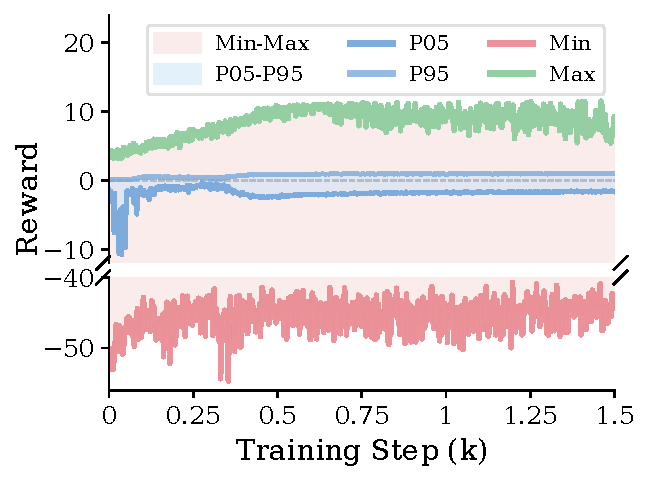
\includegraphics[width=\linewidth]{figures/fig3c_reward_extremes.pdf}\\[-0.5ex]
    \textbf{(c)}
  \end{minipage}
  \vspace{-8pt}
    \caption{
    Pathological OPD rewards. The OPD reward shows (a) high variance with a heavy negative tail, (b) early-position extreme values, and (c) persistent extremes throughout training.
    }
    \vspace{-12pt}

  \label{fig:reward-diagnosis}
\end{figure*}

\section{Preliminaries}
\label{sec:Preliminaries}

\subsection{On-Policy Distillation}
\label{sec:opd}

On-policy distillation (OPD)~\citep{agarwal2024gkd,gu2024minillm,song2026survey} has emerged as a standard stage in LLM post-training pipelines~\citep{qwen3, HY_MT1.5, glm5, nemotron2, deepseekv4, HY_Embodied_0.5, mimo_v2_flash, kat_coder_v2, Qwen3.5_Omni}. It trains a student policy $\pi_\theta$ to match a stronger teacher policy $\pi_T$ on trajectories generated by the student itself. This on-policy training reduces exposure bias by aligning the training-time contexts with the student's inference-time generation. OPD minimizes the reverse KL divergence, which encourages mode-seeking toward the teacher's dominant modes~\citep{kevin2025opd}:
\[
D_{\mathrm{KL}}(\pi_\theta \| \pi_T)
=
\mathbb{E}_{x \sim \mathcal{D},\, o \sim \pi_\theta(\cdot \mid x)}
\left[
\log
\frac{
\pi_\theta(o \mid x)
}{
\pi_T(o \mid x)
}
\right],
\]
where \(x\) is a prompt from \(\mathcal{D}\) and \(o=(o_1,\ldots,o_{|o|})\) is a student-generated response.

\subsection{OPD as Dense-Reward RL}
\label{sec:opd-as-rl}

Using the autoregressive factorization of $\pi_\theta$ and $\pi_T$, OPD maximizes the negative reverse-KL objective in the token-level form
\[
J_{\mathrm{OPD}}(\theta)
=
\mathbb{E}_{x \sim \mathcal{D},\, o \sim \pi_\theta(\cdot \mid x)}
\left[
\sum_{t=1}^{|o|}
\log
\frac{
\pi_T(o_t \mid c_t)
}{
\pi_\theta(o_t \mid c_t)
}
\right],
\]
where $c_t=(x,o_{<t})$ denotes the context before token $o_t$. Following recent practice~\citep{kevin2025opd, ko2026reopold, oh2026kl}, this objective is optimized as policy-gradient RL~\citep{williams1992reinforce, sutton1999policygrad}:
\[
\begin{aligned}
&\nabla_\theta J_{\mathrm{OPD}}(\theta)
=
\mathbb{E}_{x \sim \mathcal{D},\, o \sim \pi_\theta(\cdot \mid x)}\\
&\Bigg[
\sum_{t=1}^{|o|}
\log
\frac{\pi_T(o_t \mid c_t)}
{\pi_\theta(o_t \mid c_t)}
\nabla_\theta \log \pi_\theta(o_t \mid c_t)
\Bigg].
\end{aligned}
\]
Appendix~\ref{app:opd-pg-derivation} provides the detailed derivation. This policy-gradient form identifies the stop-gradient log-ratio term as the OPD token-level reward:
\begin{equation}
r_t^{\mathrm{OPD}}(c_t,o_t)
=
\log
\frac{
\pi_T(o_t \mid c_t)
}{
\pi_\theta(o_t \mid c_t)
}.
\label{eq:opd-token-reward}
\end{equation}
Unlike the sparse sequence-level rewards used in outcome-based RL~\citep{deepseekmath, deepseekr1}, the OPD reward is dense and depends explicitly on the current student policy $\pi_\theta(o_t \mid c_t)$.